\chapter{Fundamentos b\'asicos del procesamiento de im\'agenes}

Una vez presentadas las bases físicas que dan lugar a la formación de las imágenes radiológicas, en el presente Capítulo se introducirán los primeros conceptos básicos y la formulación matemática necesaria para un acercamiento al procesamiento de imágenes digitales. Así, se introducirá al lector en las primeras nociones para lograr comprender la representación y las operaciones elementales del procesamiento digital de imágenes.

\section{Introducción al procesamiento de imágenes}

El análisis y procesamiento de imágenes se realiza a través de computadoras, debido a la complejidad y el número de cálculos necesarios para realizarlo. Es por esto que, si bien la formulación matemática necesaria para su realización data de varios siglos atrás, la posibilidad real de utilizarla de forma cotidiana en la práctica clínica ha sido posible recién en las últimas décadas, gracias al avance en las tecnologías del hardware.

La proliferación de nuevos equipamientos con capacidad para realizar millones de operaciones por segundo y su extensión a la vida cotidiana y a todo tipo de usuario, ha hecho posible que el análisis y procesamiento de imágenes digitales se constituya en un gran campo de estudio. En la actualidad, esta tecnología se encuentra incorporada incluso en todo tipo de equipamiento doméstico, como cámaras digitales, scaners y teléfonos celulares, entre otros.

En términos históricos, la utilización de imágenes radiográficas para diagnóstico clínico data prácticamente desde el descubrimiento de los rayos X en 1895 (Röentgen). Incluso, las imágenes funcionales a partir de la emisión de fotones (rayos $\gamma$) por parte de radionucleidos ya cuenta con más de 90 años de antigüedad (Heavesy \& Seaborg, 1924). Sin embargo, las imágenes eran adquiridas sobre films radiográficos o directamente \emph{in vivo}, por lo que su correcto procesamiento no ha explotado su real potencialidad sino hasta la incorporación de la tecnología que permitió digitalizarlas.

El motivo principal de esta ``aparición tardía'' del procesamiento de imágenes ha sido entonces, debido a los requerimientos de hardware tanto para el procesamiento de las mismas como para la representación de estas en sistemas gráficos de alta performance. Paralelamente a este desarrollo, la formulación de algoritmos para el procesamiento ha seguido los avances tecnológicos logrando un alto grado de sofisticación y manipulación de imágenes en tiempo casi real.

La variedad actual de técnicas, algoritmos y desarrollos de software y hardware utilizados en el procesamiento de imágenes digitales escapa al alcance de cualquier curso. En ellos se aprovechan técnicas desarrolladas inicialmente sobre conceptos fundacionales para el análisis de imágenes, y se incorporan conceptos y nociones de los más variados, propios de la física y la matemática, como el caso de la entropía o la métrica.

En el presente capítulo se introducirán las primeras nociones y conceptos para abordar el estudio del procesamiento de imágenes digitales, entre los que se cuentan las formatos de lectura y representación de imágenes, las operaciones de modificación, las transformaciones sobre tonalidades y colores, y la generación de efectos sobre regiones de una imagen.

El interés del siguiente estudio puede condensarse en dos objetivos principales: a) lograr una mejora considerable de la calidad de la imagen para la interpretación de un especialista, y/o b) lograr la obtención de información específica para su procesamiento por medio de sistemas de cálculo y análisis.

Serán de interés de este curso, las imágenes producidas por interacción de la radiación ionizante con la materia para uso médico, es decir aquellas adquiridas por detectores de rayos X o $\gamma$\footnote{Se entiende como rayos X a aquellos producidos en interacciones atómicas, y rayos $\gamma$ a aquellos producidos por interacciones internucleares. No existe \emph{a priori} diferencia energética entre ellos y ambos son constituidos por fotones, la diferencia se realiza a partir de su procedencia. En adelante se utilizará indistintamente las letras X o $\gamma$ para referirse a fotones.} y que hayan atravesado -o partido de- tejido biológico de un paciente, formando una imagen bidimensional (2D) o tridimensional (3D).


\section{Formato de imagen y representación digital}

En la actualidad, las imágenes constituyen un lenguaje en sí mismas. Dependiendo de diferentes factores culturales, las imágenes son utilizadas para transmitir mensajes, símbolos y distintos tipos de información. Por esto, es necesario contar con un soporte para la representación digital de las imágenes que permita luego modificar el mismo a fin de o bien modificar el contenido visual y simbólico u obtener información necesaria.

  \subsection{Bandas en imágenes digitales}
  
  Para lograr adquirir una imagen, de forma remota, debe existir algún tipo de interacción entre el objeto que se desea observar y el detector. En las imágenes digitales, los distintos tipos de detector dependen del tipo de radiación electromagnética que son capaces de detectar. Así como la información que se puede obtener de un objeto depende también de la interacción de esta radiación con el objeto. De esta particularidad proviene el concepto de ``bandas'', donde se divide el espectro electromagnético en función de los tipos de interacción de la radiación con la materia (ver Fig. \ref{fig2-1}), lo que define desde los objetos a analizar hasta los detectores y materiales que pueden utilizarse.
  
  Todos los objetos absorben, reflejan o emiten cuantos de energía dependiendo de su longitud de onda, intensidad y tipo de radiación. Este tipo de radiación se define a partir de sus propiedades físicas dentro del espectro electromagnético. El ojo humano, por su parte, solo es capaz de detectar energía electromagnética en el espectro de luz visible, mientras que para los rayos X, la radiación ultravioleta, infrarroja o de microondas, es necesaria la construcción de detectores que puedan recabar esta información, ya sea de forma digital o analógica, para poder ser cuantificada y analizada.
  
  \begin{figure}
   \centering
   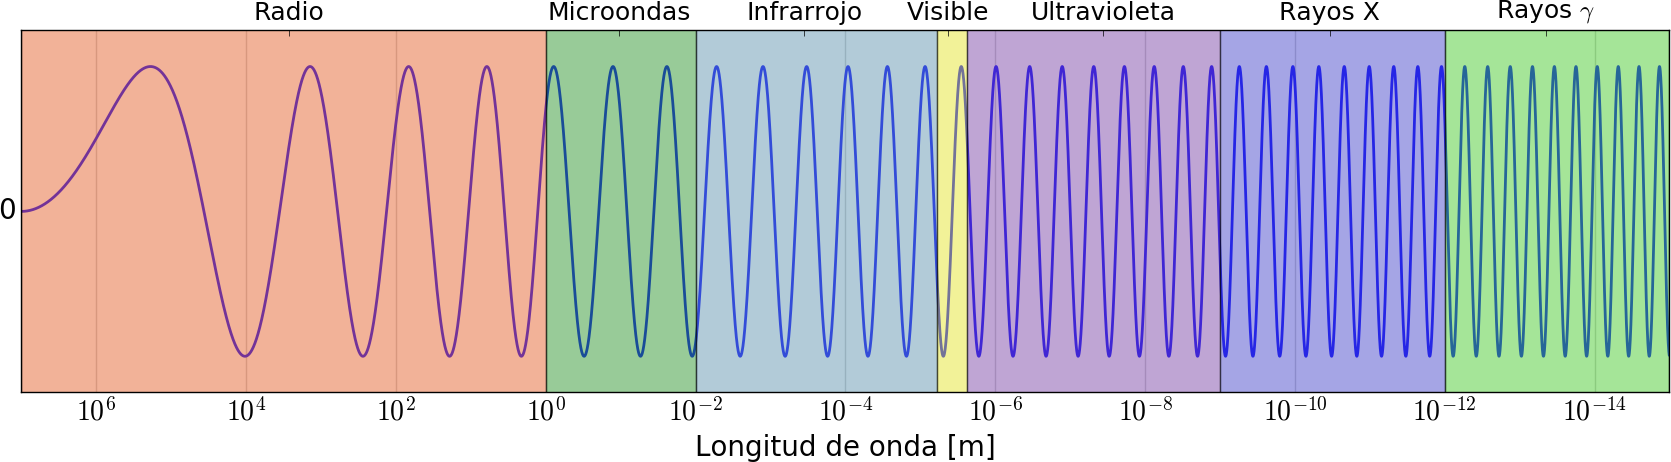
\includegraphics[width=\textwidth]{figures/cap2/fig1_bandas/figure_1.png}
   \caption{Esquema cualitativo del espectro electromagnético}
   \label{fig2-1}
  \end{figure}

  \vfill
  
%   \subsection{Representación digital}
%   
%   
%     \subsubsection{Mapa de bits}
%   
%     \subsubsection{Imágenes vectoriales}
%   
%   \subsection{Modificación sobre colores}
%   
%   \subsection{Histograma de una imagen}
%   
%   \subsection{Resolución de una imagen}
%   
%   \subsection{Resolución, tamaño de imagen, tamaño de archivo}
%   
%   \subsection{Contraste en una imagen}
%   
% \section{Vínculo físico del origen de las imágenes}
% 
% \section{Modificación de una imagen}
% 
%   \subsection{Corrección \(\gamma\): colores y tonalidades}
%   
%   \subsection{Inversión (\emph{flip})}
%   
%   \subsection{Reflección (\emph{mirror})}
%   
%   \subsection{Interpolación}
%   
%   \subsection{Comparación cualitativa de algoritmos}
% 
% \section{Relaciones básicas entre píxeles}
% 
% \section{Operaciones sobre imágenes}
% 
% \section{Operaciones sobre píxeles}
% 
% \section{La transforma discreta de Fourier}
% 
% \section{Filtros}
% 
%   \subsection{Filtros de paso de banda}
%   
%   \subsection{Filtros de suavizado}
%   
%   \subsection{Máscaras de filtrado}

\subsection{Representaci\'on digital: mapa de bits (Bitmaps)}
% \markboth{Intr. proc. im\'agenes radiol\'ogicas \'ambito m\'edico \ \textbf{M\'ODULO II}}{ESPECIALIDAD III \ \textbf{M\'ODULO II}}

Un Bitmap es un modo elemental para representar im\'agenes digitales como informaci\'on en el \textit{hardware}, espec\'ificamente la memoria, de un
computador.
%
Consiste, b\'asicamente, en formar arreglos de elementos (vectores, matrices, tensores) ordenados de modos espec\'ificos.
%
En general, para el caso t\'ipico de im\'agenes 2D, se realiza un ordenamiento por filas de elementos de matriz (\textit{pixels}) asignando a cada uno 
un valor que determina ``el color'' en esa posici\'on de la imagen.
%

%
En el caso de im\'agenes en tonalidades de grises, el valor del elemento de matriz es un escalar; mientras que para el caso de im\'agenes a color el 
valor de cada elemento de matriz es un vector de tres coordenadas, cada una de las cuales especifica ``el grado de influencia'' de los colores rojo 
(Red ``R''), verde (Green ``G'') y azul (Blue ``B''), de modo que se denomina representaci\'on RGB). 
%
Existen otros modos de representaci\'on a color, como por ejemplo CMYK (ci\'an, magenta, amarillo y negro). 
%

%
T\'ipicamente se emplean escalas (que determinan ``rangos din\'amicos'') en $2^{N}$ bits, y se denomina $N-$ bits. Es decir, para el caso m\'as com\'un de 
8-bits, la escala es $[0, 255]$, ya que por costumbre se define el rango como $[0, 2^{N} - 1]$. 
%

%
El uso t\'ipico de 8-bits est\'a basado, principalmente, en dos motivos. En primer lugar, estudios biom\'etricos muestran que el ojo humano no
es suficientemente sensible para diferenciar m\'as de 256 niveles de intensidad para un dado color. Adem\'as, el rango de valores para los 
elementos de matriz determinan las necesidad en cuanto a la capacidad de almacenamiento en el computador.
%

%
Entonces, para im\'agenes en tonalidades de grises, conocidas
como ``de una banda'' el rango para los valores de los elementos de matriz (escalares) es $[0, 255]$, mientras que para im\'agenes a color, los valores de 
elementos de matriz (vectores de 3 coordenadas) asumen valores en $([0, 255], [0, 255], [0, 255])$.
%
Si embargo, tambi\'en es frecuente encontrar representaciones 
normalizadas para im\'agenes a color, es decir, elementos de matriz en $([0, 1], [0, 1], [0, 1])$ para determinar los colores RGB.
%

%
Todos los colores en el rango visible pueden representarse como combinaciones RGB, variando desde el negro $(0, 0, 0)$ al blanco $(255, 255, 255)$.
%
Por lo tanto, una imagen RGB es representada por un arreglo bidimensional de \textit{pixels}, cada uno codificado en 3 bytes pudiendo asumir 
$256^{3}$ diferentes valores de combinaciones vectoriales, es decir 16.8 millones de diferentes colores, aproximadamente.
%

\subsection{Representaci\'on digital: im\'agenes vectoriales}
% \markboth{Intr. proc. im\'agenes radiol\'ogicas \'ambito m\'edico \ \textbf{M\'ODULO II}}{ESPECIALIDAD III \ \textbf{M\'ODULO II}}

Las im\'agenes vectoriales est\'an constituidas por contornos y rellenos definidos matem\'aticamente, vectorialmente,  por medio de ecuaciones que 
describen perfectamente cada ilustraci\'on. 
%
De este modo, es posible implementar \textit{scaling} sin p\'erdida de calidad.
%
El proceso de \textit{scaling} es t\'ipico en la formaci\'on, producci\'on o reproducci\'on en dispositivos. Por ello, la importancia de mantener la 
invariabilidad. 
%
Esta caracter\'istica resulta de particular relevancia en casos que las ilustraciones contengan marcadas zonas con contornos curvados, ya que el pixelado 
implicar\'ia una p\'erdida de resoluci\'on, como indica la figura .

%

\begin{center}
\begin{figure} [!h]

\centering
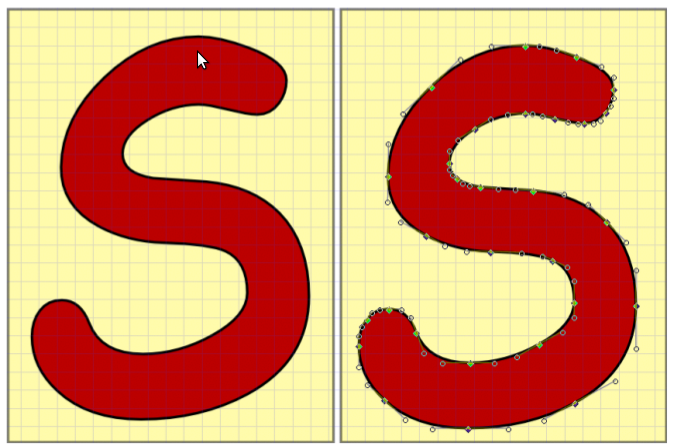
\includegraphics[width=12cm]{Figuras/Fig2_1.png}
   
\caption{Imagen en representaci\'on vectorial (izquierda) y en pixelado bitmap (derecha).}
\label{Fig2_1}

\end{figure}
\end{center}



\subsection{Modificaci\'on de colores en im\'agenes}
% \markboth{Intr. proc. im\'agenes radiol\'ogicas \'ambito m\'edico \ \textbf{M\'ODULO II}}{ESPECIALIDAD III \ \textbf{M\'ODULO II}}


Es posible cuantificar la diferencia entre dos colores (en representaci\'on digital, valores del trio vectorial RGB) calculando la distancia, seg\'un alg\'un 
tipo de m\'etrica, Euclidea por ejemplo, entre los vectores que los representan.
%

%
Se el color $C_{1}$ representado por el vector $(R_{1}, G_{1}, B_{1})$ y el color $C_{2}$ representdo por $(R_{2}, G_{2}, B_{2})$.
%
Entonces, en el espacio vectorial, la distancia $D (C_{1}, C_{2})$ entre \'estos est\'a dada por:

%

\begin{eqnarray}
	D(C_{1}, C_{2}) = \sqrt{ \left(R_{1} - R_{2} \right)^{2} + \left(G_{1} - G_{2} \right)^{2} + \left(B_{1} - B_{2} \right)^{2}}
\label{EqXXII}
\end{eqnarray}

Para el caso particular de im\'agenes de una banda (tonalidades de grises) puede aplicar la misma metodolog\'ia descrita para im\'agenes RGB con la 
simplificaci\'on asociada al hecho de que en el espacio de colores, los vectores en la direcci\'on del vector $(1, 1, 1)$ representan
las diferentes tonalidades de gris. 
%

%
Por tanto, existe la equivalencia de que para cualquier \textit{pixel} de tipo RGB $(R, G, B)$ si se lo proyecta sobre $(1, 1, 1)$ se obtiene la 
contribuci\'on de cada tonalidad de gris.
%
Entonces, se tiene:

\begin{eqnarray}
	Proy \equiv (R, G, B) \cdot (1, 1, 1) =R + G + B = \lvert \vec{V} \rvert \lvert \hat{n} \rvert cos(\phi)
\label{EqXXIIb}
\end{eqnarray}

donde $Proy$ es la proyecci\;\'on, $\vec{V}$ es el vector que forma el punto $(R, G, B)$ en el espacio de coordenadas del tr\'io (representaci\'on vectorial),
$\hat{n}$ es el versor de proyecci\'on $(1, 1, 1)$ y $\phi$ es el \'angulo que forma $\vec{V}$ con $\hat{n}$.
%

%
De aqu\'i puede verse que $Proy = \frac{R + G + B}{\sqrt{3}}$ y debe atenderse de que este valor no exceda 255, de modo que es usual renormalizar para 
obtener $Proy = \frac{R + G + B}{3}$

\vspace{1.0cm}


\begin{center}

\underline{Ejemplo de modificaci\'on de colores: Por detecci\'on de bordes}

\end{center}

A modo de ilustraci\'on de los conceptos generales expuestos sobre representaciones vectoriales-bitmap, se propone un caso de aplicaci\'on muy sencillo.
%
Si el objetivo en la detecci\'on de bordes (orillas) de las formas en una imagen para obtener el bitmap resultante que resalte los bordes 
en blanco-negro, puede procederse del siguiente modo: Desplazarse dentro de la imagen \textit{pixel} a \textit{pixel} comparando el color de cada uno 
con su vecino de la derecha y su vecino de abajo. 
%
Luego, se efect\'ua el siguiente control (criterio): si al comparar resulta en una diferencia muy 
grande (``muy grande'' es un par\'ametro\footnote{Este par\'ametro es denominado ``umbral'' y su valor condiciona la \textit{performance} de la t\'ecnica.} 
o conjunto de par\'ametros pre-definidos por el usuario, o bien automatizados en casos m\'as elaborados) 
el \textit{pixel} en consideraci\'on forma parte del borde y se le asigna el color blanco, de otro modo se asigna el color negro.
%

\subsection{Histograma de una imagen}
% \markboth{Intr. proc. im\'agenes radiol\'ogicas \'ambito m\'edico \ \textbf{M\'ODULO II}}{ESPECIALIDAD III \ \textbf{M\'ODULO II}}

Dada la representaci\'on digital de una imagen por medio del arreglo de $N$ filas por $M$ columnas se determina una matriz $M \times N$, en la cual la 
representaci\'on digital de bitmap estar\'a dada por la funci\'on distribuci\'on $f(m, n)$, para $n \in [0, N-1]$ y $m \in [0, M-1]$, t\'ipicamente
$N$ y $M$ son potencias de 2, como ya se enunci\'o.
%

%
El histograma de una imagen $h(i)$, com\'unmente denominado \textit{``image enhancenment''} o \textit{``image characterization''} es un vector que da cuenta de 
la cantidad de \textit{pixels} dentro de la imagen con un cierto valor de elemento.
%
Es decir, para una imagen de $\alpha$-bits, se tiene:
%

\begin{eqnarray}
	h(i) \equiv \sum _{m=0}^{M-1} \, \; \sum _{n=0}^{N-1} \delta(f(n, m) - i) \; \, \; \forall i \in [0, 2^{\alpha}-1]
\label{EqXXIII}
\end{eqnarray}

%
Una de las t\'ecnicas gen\'ericas, que luego se diversifica a una cantidad muy variada de metodolog\'ias espec\'ificas de procesamiento, es el m\'etodo de 
convoluci\'on.
%
Sea $w(k, l)$ un arreglo $2 \times K + 1, 2 \times L + 1$, centrado en el ``origen'' $(0, 0)$ que coincide con el \textit{pixel} central de la imagen.
%
Puede considerarse a $w(k, l)$ como un \textit{kernel} de convoluci\'on de modo que aplicado a la imagen $f(n, m)$ resulte:
%

\begin{eqnarray}
	g(m, n) \equiv w(k, l) \ast f(m, n) = \sum _{k=-K}^{K} \, \; \sum _{l=-L}^{L} w(k, l) \cdot f(m-k, n-l)
\label{EqXXIV}
\end{eqnarray}

A partir de esta definici\'on, pueden introducirse una gran cantidad de m\'etodos espec\'ificos, entre los que se destacan las transformadas, como Fourier, 
Laplace, Radon, etc.


\subsection{Resoluci\'on de una imagen}
% \markboth{Intr. proc. im\'agenes radiol\'ogicas \'ambito m\'edico \ \textbf{M\'ODULO II}}{ESPECIALIDAD III \ \textbf{M\'ODULO II}}
%
\textit{A priori}, este concepto tiene diferentes acepciones seg\'un el contexto en el que se utilice y se podr\'ia definir, de modo gen\'erico, como
la capacidad para representar o percibir los detalles de una imagen.
%
Se trata de un concepto presente en todo el proceso digital, desde la captura o generaci\'on hasta la representaci\'on, y afecta (condiciona) el 
procesamiento posterior.
%

%
Una definici\'on \'util es: la resoluci\'on de una imagen es la cantidad de \textit{pixels} que la describen. 
%
Y una medida t\'ipica es en t\'erminos de ``\textit{pixels} por pulgada'' (ppi). 
%
Por tanto, la calidad de la representaci\'on as\'i como el tama\~no de la imagen dependen de la resoluci\'on, que determina a su vez los reqerimientos 
de memoria para el archivo gr\'afico a generar.


\subsection{Resoluci\'on, tama\~no de imagen y tama\~no de archivo}
% \markboth{Intr. proc. im\'agenes radiol\'ogicas \'ambito m\'edico \ \textbf{M\'ODULO II}}{ESPECIALIDAD III \ \textbf{M\'ODULO II}}

Los tres conceptos est\'an estrechamente relacionados y dependen mutuamente, aunque se refieren a caracter\'isticas diferenciadas y debe evitarse 
la confusi\'on.
%

%
El tama\~no de una imagen son sus dimensiones reales en t\'erminos de anchura y altura una vez impresa, mientras que el tama\~no del archivo se refiere a la 
cantidad de memoria f\'isica necesaria para almacenar la informaci\'on de la imagen digitalizada en cualquier soporte inform\'atico de almacenamiento.
%

%
Ciertamente, la resoluci\'on de la imagen condiciona fuertemente estos dos conceptos, ya que la cantidad de \textit{pixels} de la imagen digitalizada es 
fijo y por tanto al aumentar el tama\~no de la imagen se reduce la resoluci\'on y viceversa. 
%

%
A modo de ejemplo: duplicando la resoluci\'on de una imagen digitalizada, de 50 ppi a 100 ppi, el tama\~no de la imagen se reduce a la cuarta parte del 
original mientras que dividir la resoluci\'on por 2. Es decir, se pasa de 300 ppi a 150 ppi obteniendo una imagen con el doble de las dimensiones originales
que represebtan cuatro veces su superficie.
%

%
La reducci\'on de la resoluci\'on de la imagen, manteniendo su tama\~no, provoca eliminaci\'on de \textit{pixels}.
%
Entonces, se obtiene una representaci\'on (descripci\'on) menos precisa de la imagen, as\'i como transiciones de color m\'as bruscas. 
%
El tama\~no del archivo que genera una imagen digitalizada es proporcional, como se espera, a la resoluci\'on, por lo tanto, variarla implica modificar
en el mismo sentido el tama\~no del archivo.

\subsection{Contraste en una imagen}
% \markboth{Intr. proc. im\'agenes radiol\'ogicas \'ambito m\'edico \ \textbf{M\'ODULO II}}{ESPECIALIDAD III \ \textbf{M\'ODULO II}}

Conceptualmente, aumentar o disminuir el contraste en una imagen consiste, b\'asica y visualmente, en aumentar o disminuir la pendiente de la linea recta 
con pendiente a 45 grados que representa los grises (con la precauci\'on de no exceder los l\'imites 0-255) entre \textit{input} y \textit{output}, como 
indica la figura \ref{Fig2_2}.
%

%
La transformaci\'on correspondiente al cambio de contraste es:

\begin{eqnarray}
	V_{O}(m, n) = \left( V_{I}(m, n) - 2^{Y - 1} \right) \, \tan{\phi} \, + 2^{Y - 1}
\label{EqXXV}
\end{eqnarray}

donde $Y$ es la escala en bits, $V_{I}$ y $V_{O}$ son los valores de \textit{input} y \textit{output}, respectivamente valuados en el pixel $(m, n)$; y el \'angulo $\phi$ cooresponde a 
las propiedades de la transformaci\'on lineal de contrastes, espec\'ificamente la pendiente (figura \ref{Fig2_2}).

%

\begin{center}
\begin{figure} [!h]

\centering
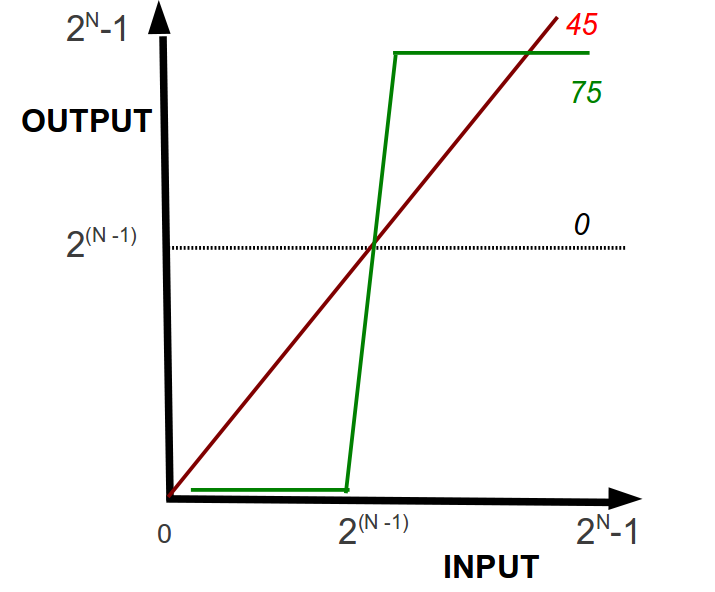
\includegraphics[width=10cm]{Figuras/Fig2_2.png}
   
\caption{Representaci\'on del cambio de contraste entre \textit{input} y \textit{output}.}
\label{Fig2_2}
\end{figure}
\end{center}

%
\section{V\'inculo f\'isico del origen de im\'agenes}
% \markboth{Intr. proc. im\'agenes radiol\'ogicas \'ambito m\'edico \ \textbf{M\'ODULO II}}{ESPECIALIDAD III \ \textbf{M\'ODULO II}}

Las im\'agenes generadas por radiaci\'on electromagn\'etica pueden clasifcarse en modo gen\'erico seg\'un el ordenamiento de mayor a menor frecuencia.

\begin{description}
 \item[Rayos $\gamma$] medicina nuclear, observaciones de astronom\'ia.
 \item [Rayos X] diagn\'ostico m\'edico e industria (control de calidad).
 \item[Banda ultravioleta] Inspecci\'on industrial y microscop\'ia biol\'ogica.
 \item[Banda visible e infrarroja] Aplicaciones varias, fotograf\'ia.
 \item[Microondas] radar.
 \item[Ondas de radio] medicina (MRI) y algunas aplicaciones en astronom\'ia. 
\end{description}



\section{Modificaci\'on de una imagen}
% \markboth{Intr. proc. im\'agenes radiol\'ogicas \'ambito m\'edico \ \textbf{M\'ODULO II}}{ESPECIALIDAD III \ \textbf{M\'ODULO II}}

Una imagen \textit{input} puede ser modifica por medio de diferentes maneras, seg\'un la/s propiedad/es que se modifica/n.
%

%
En particular, se consideran a continuaci\'on algunas de las modificaciones m\'as frecuentes.

\subsection{Modificaci\'on de colores o tonalidades: Correcci\'on $\gamma$}
\markboth{Intr. proc. im\'agenes radiol\'ogicas \'ambito m\'edico \ \textbf{M\'ODULO II}}{ESPECIALIDAD III \ \textbf{M\'ODULO II}}

Existe una amplia variedad de t\'ecnicas y criterios para modificar los colores de una imagen.
%
Una de las metodolog\'ias m\'as empleada, y sencilla, es la correcci\'on $\gamma$, definida a partir de:

\begin{eqnarray}
	V_{O}(m, n) = \left( 2^{N} - 1 \right) \left( \frac{V_{I}(m, n)}{2^{N} -1} \right)^{\frac{1}{\gamma}}
\label{EqXXVI}
\end{eqnarray}

donde el \'indice $\gamma$ asume valores $\in \Re$.
%

%
Por lo tanto, resulta:

\begin{itemize}
 \item Para $\gamma$ = 1 no hay ninguna correcci\'on.
 \item Para valores de $\gamma > 1$ hay una gran correcci\'on en el contraste para valores peque\~nos del color de \textit{input} mientras que una 
 peque\~na correcci\'on en el contraste para valores altos. El brillo aumenta m\'as para valores intermedios del color de \textit{input}.
 \item Para valores de $\gamma < 1$ hay una peque\~na correcci\'on en el contraste para valores bajos del color de \textit{input}, mientras que una 
 gran correcci\'on en el contraste para valores altos. El brillo disminuye m\'as para valores intermedios del color de \textit{input}.
\end{itemize}


\subsection{Modificaci\'on de imagen: inversi\'on (\textit{flip})}
% \markboth{Intr. proc. im\'agenes radiol\'ogicas \'ambito m\'edico \ \textbf{M\'ODULO II}}{ESPECIALIDAD III \ \textbf{M\'ODULO II}}

B\'asicamente, esta modificaci\'on consiste en una transformaci\'on que 
produce un  ``movimiento'' de la columna $m$, fila $n$ a la columna $m$ y 
fila $(n_{max} - n) + 1$, para $n_{max}$ como la dimensi\'on en la 
direcci\'on de $n$.
%

%
Es decir,

\begin{eqnarray}
	V_{flip}(m, n) = V_{I} (m, (n_{max} - n) + 1)
\label{EqXXVII}
\end{eqnarray}

donde $V_{flip}$ es la matriz de output que corresponde a la transformaci\'on de inversi\'on.

\subsection{Modificaci\'on de imagen: reflexi\'on (\textit{mirror})}
% \markboth{Intr. proc. im\'agenes radiol\'ogicas \'ambito m\'edico \ \textbf{M\'ODULO II}}{ESPECIALIDAD III \ \textbf{M\'ODULO II}}

B\'asicamente, esta modificaci\'on consiste en una transformaci\'on que produce un  ``movimiento'' de la fila $n$, columa $m$ a la fila $n$ y 
columna $(m_{max} - m) + 1$, para $m_{max}$ como la dimensi\'on en la 
direcci\'on de $m$.
%

%
Es decir,

\begin{eqnarray}
	V_{mirror}(m, n) = V_{I} ((m_{max}  - m) + 1, n)
\label{EqXXVIII}
\end{eqnarray}

donde $V_{mirror}$ es la matriz de output que corresponde a la transformaci\'on de reflexi\'on.

\subsection{Modificaci\'on de imagen: interpolaci\'on}
% \markboth{Intr. proc. im\'agenes radiol\'ogicas \'ambito m\'edico \ \textbf{M\'ODULO II}}{ESPECIALIDAD III \ \textbf{M\'ODULO II}}

A partir de de un muestreo \textit{input} pueden estimarse los valores de la intensidad en puntos diferentes a aquellos puntos donde si se conoce el valor 
%
Entre otras t\'ecnicas, se destacan los m\'etodos de \textit{re-sampling}.
%

%
De este modo, se emplean diferentes criterios para determinar los valores $V_{O}(k, l)$ para \textit{pixels} $(k, l)$ donde el \textit{input} $V_{I}$ no es 
conocido:

\begin{itemize}
 \item Interpolaci\'on al vecino m\'as cercano.
 \item Interpolaci\'on bilineal.
 \item Interpolaci\'on bic\'ubica.
\end{itemize}

La t\'ecnica de interpolaco\'on al vecino m\'as cercano (\textit{Nearest neighbor interpolation}) est\'a basada en superponer el arreglo 2D \textit{output}
al arreglo 2D \textit{input} calculando el valor para los \textit{pixels} $(k, l)$ seg\'un los valores conocidos $V_{I}(i, j)$, utilizando un promedio 
(que puede cuantificarse de diferentes maneras) de 
los vecinos m\'as cercanos equidistantes. 
%
Sin embargo, puede verse que esta t\'ecnica presenta algunos efectos indeseables.
%

%
La t\'acnica de interpolaci\'on lineal considera los 4 \textit{pixels} m\'as cercanos a $V(k, l)$ para la interpolaci\'on.
%
Se realiza un promedio entre estos 4 valores para determinar el valor desconocido del \textit{pixel} $(k, l)$.
%
La imagen \textit{output} resulta m\'as ``suave'' que para el caso de la t\'ecnica \textit{Nearest neighbor interpolation}.
%
Pero, puede causar que la imagen se vea algo ``difusa''.
%

%
Entonces, los valores de \textit{pixels} $(k, l)$, para los cuales no se conoce $V_{I}(k, l)$ se obtienen a partir de:


\begin{eqnarray}
	V_{O}(k, l) = (1 - \alpha)\, (1-\beta) \, V_{I}(i,j) + \alpha (1 - \beta) \, V_{I}(i +1, j) + \nonumber \\
	(\alpha -1) \, V_{I}(i, j+1) + \alpha \, \beta \, V_{I}(i +1, j +1)
\label{EqXXIX}
\end{eqnarray}

donde $\alpha \equiv k - i$, $\beta \equiv l -j$, $i \equiv floor(k)$ y $j \equiv floor(l)$\footnote{Aqu\'i la funci\'on \textit{floor}
se define por medio de asignar al argumento el n\'umero entero m\'as grande que sea menor que el argumento.}.


Por su parte, la t\'ecnica de interpolaci\'on bic\'ubica Es el algoritmo de interpolaci\'on m\'as utilizado.
%
Considera los 16 \textit{pixels} m\'as cercanos a cada \textit{pixel} $(k, l)$ cuyo valor debe determinarse por interpolaci\'on.
%
Se aproxima localmente al valor (el nivel de gris) en la imagen original mediante una superficie polin\'omica de tipo bic\'ubica.
%
Resulta ser, de las t\'ecnicas qu\'i descritas, el \'optimo al considerar el balance entre tiempo de c\'omputo y \textit{performance}.
%

%
La implementaci\'on de este m\'etodo puede llevarse a cabo por medio de
procesar el bloque $B(k, l)$, centraado en el \textit{pixel}
$(k, l)$, cuyas dimensiones se corresponden con las dimensiones de la m\'ascara 
(16 \textit{pixels} en un arreglo 5 $\times$ 5): 

\begin{eqnarray}
	B(k, l) = \sum _{i=0}^{3} \sum _{j=0}^{3} \, 
q^{(k, l)}_{i, j} (k - k')^{i} \, (l - l')^{j} \\ \nonumber
\, \, \; \; k', \,  \in [k - 2, k + 2] \; \, \& \; 
l' \,  \in [l - 2, l + 2]
\label{EqXXX}
\end{eqnarray}

donde los coeficientes $q_{i, j}$ deben ser determinados. 
%
O bien, 

\begin{eqnarray}
	V_{O}(k, l) = h(k) \, h(l) 
\label{EqXXXI}
\end{eqnarray}


donde la funci\'on de interpolaci\'on $h$ se define, a trozos, del siguiente modo:

\begin{eqnarray}
	h(p) \equiv 1 - \, \lvert p \rvert^{2} + \lvert p \rvert^{3} \; \, \; \forall \lvert p \rvert < 1 \nonumber \\
	h(p) \equiv 4 - \, 8 \, \lvert p \rvert^{2} + 5 \, \lvert p \rvert^{2} - \lvert p \rvert^{3} \; \, \; \forall 1 \leq \lvert p \rvert < 2 \\
	h(p) \equiv 0 \, \; \, \forall p \geq 2 \nonumber
\label{EqXXXII}
\end{eqnarray}


\subsection{Comparaci\'on cualitativa de performance de algoritmos de  interpolaci\'on}
% \markboth{Intr. proc. im\'agenes radiol\'ogicas \'ambito m\'edico \ \textbf{M\'ODULO II}}{ESPECIALIDAD III \ \textbf{M\'ODULO II}}

\begin{itemize}
 \item Interpolaci\'on de vecino m\'as cercano: El error de posici\'on resulta, a los sumo, medio \textit{pixel}, que es perceptible en objetos con
fronteras rectas en las que aparece un efecto de salto despu\'es de de esta transformaci\'on.
 \item Interpolaci\'on Lineal: Genera una leve disminuci\'on de resoluci\'on debido al borroneo (\textit{blurring}) intr\'inseco al modo de c\'alculo 
 del valor promedio, pero disminuye el efecto de salto que presenta el algoritmo de vecino m\'as cercano.
 \item Interpolaci\'on Bic\'ubica: No presenta el problema del efecto de salto a la vez que genera un menor \textit{blurring}.
\end{itemize}


\section{Relaciones b\'asicas entre pixels}
% \markboth{Intr. proc. im\'agenes radiol\'ogicas \'ambito m\'edico \ \textbf{M\'ODULO II}}{ESPECIALIDAD III \ \textbf{M\'ODULO II}}

La relaci\'on b\'asica m\'as inmediata entre \textit{pixels} es la distancia $D$ entre dos \textit{pixels} $(m, n)$ y $(m', n')$.
%

Los axiomas para definir una m\'etrica o funci\'on de distancia entre \textit{pixels} $D$ requieren de los siguientes criterios:

\begin{itemize}
 \item $D(k \; k', l \; l') \geq 0$ con $D(k \; k', l \; l') = 0 \Leftrightarrow k=k' \, \; l=l'$
 \item $D(k \; k', l \; l') = D(k' \; k, l' \; l)$
 \item $D(k \; k', l \; l') \leq D(k \; k', s \; s') + D(s \; s', l \; l')$
\end{itemize}

A partir de estas condiciones pueden definirse diferentes m\'etricas. Entre ellas:

\begin{center}
 \underline{Distancia Euclidea}


\begin{eqnarray}
	D(k \; k', l \; l') \equiv \sqrt{\left( k - k' \right)^2 + \left( l - l' \right)^2}
\label{EqXXXIII}
\end{eqnarray}

 \underline{Distancia $D_{4}$}


\begin{eqnarray}
	D_{4}(k \; k', l \; l') \equiv \lvert k - k' \rvert + \lvert l - l' \rvert
\label{EqXXXIV}
\end{eqnarray}

 \underline{Distancia $D_{8}$}


\begin{eqnarray}
	D_{8}(k \; k', l \; l') \equiv \max \left( \lvert k - k' \rvert , \lvert l - l' \rvert \right)
\label{EqXXXIV}
\end{eqnarray}

\end{center}

Las definiciones Euclidea, $D_{4}$ y $D_{8}$ para la distancia entre \textit{pixels} no depende de adyacencias sino exclusivamente de las coordenadas 
espaciales $(k, l)$.
%

%
Puede verse, a partir de las definiciones de las m\'etricas que la condici\'on $D(k \, k', l \, l') \leq. R$ determina un c\'irculo centrado en $(k, l)$ 
para la m\'etrica Euclidea, un rombo para la m\'etrica $D_{4}$ y un cuadrado para la m\'etrica $D_{8}$.


\section{Operadores sobre im\'agenes}
% \markboth{Intr. proc. im\'agenes radiol\'ogicas \'ambito m\'edico \ \textbf{M\'ODULO II}}{ESPECIALIDAD III \ \textbf{M\'ODULO II}}

Para operar sobre im\'agenes pueden utilizarse herramientas basadas en operaciones matriciales de \'algebra lineal y operaciones ``de array'' orientadas 
\textit{pixel a pixels}.
%
$\mathbf{H}$ es un operador arbitrario sobre una imagen cuya representaci\'on matricial es $f(m, n)$ si satisface:

\begin{eqnarray}
	\mathbf{H} \left[ f(m, n) \right] = g(m, n)
\label{EqXXXV}
\end{eqnarray}

Adem\'as, $\mathbf{H}$ es un operador lineal si:

\begin{eqnarray}
	\mathbf{H} \left[ \sum _{j} \alpha_{j} f_{j}(m, n) \right] = \sum _{j} \alpha_{j} \; \mathbf{H} \left[ f_{j}(m, n) \right]
\label{EqXXXVI}
\end{eqnarray}

Una aplicaci\'on importante de las propiedades de linealidad de operadores sobre im\'agenes es la descripci\'on de im\'agenes $g(m, n)$ como contribuci\'on 
``original'' ($f(m, n)$) y ruido \textit{random} ($r(m, n)$):

\begin{eqnarray}
	g(m, n) = f(m, n) + r(m, n)
\label{EqXXXVII}
\end{eqnarray}


La imagen de ruido es de tipo \textit{random} si los valores de \textit{pixels} de $r(m, n)$ son aleatorios no correlacionados y con esperanza 0.
%

%
Promediando $N_{Tot}$ im\'agenes con ruido \textit{random} se obtiene la imagen promedio $\langle g \rangle$ dada por:

\begin{eqnarray}
	\langle g \rangle (m, n) = \frac{1}{N_{Tot}} \sum _{j=1} ^{N_{Tot}} g_{j} (m, n) 
\label{EqXXXVIII}
\end{eqnarray}

La aplicaci\'on del teorema del l\'imite central establece que la imagen promedio $\langle g \rangle (m, n) \; \rightarrow f(m, n)$ (imagen ``original'') 
para $N_{Tot} \rightarrow \infty$.
%

%
Otra aplicaci\'on \'util de los operadores lineales es la substracci\'on de una m\'ascara\footnote{Un ejemplo t\'ipico son las im\'agenes m\'edicas por 
contraste, como angiograf\'ias.} $M(m, n)$ a la imagen original $f(m, n)$:

\begin{eqnarray}
	g (m, n) = f(m, n) - M(m, n)
\label{EqXXXIX}
\end{eqnarray}


\subsection{Adici\'on y diferencia de im\'agenes}
% \markboth{Intr. proc. im\'agenes radiol\'ogicas \'ambito m\'edico \ \textbf{M\'ODULO II}}{ESPECIALIDAD III \ \textbf{M\'ODULO II}}

Para ejemplificar las operaciones, se utilizan im\'agenes 8-bits.
%

%
Por tanto, los valores de la imagen resultado de la adici\'on de dos im\'agenes var\'ian en $[0, 510]$.
%
Mientras que los valores de la imagen resultado de la diferencia de dos im\'agenes var\'ian en $[-255, 255]$.
%

%
La adecuaci\'on ($f_{A}$) de los valores de la imagen resultado de adici\'on/diferencia de dos im\'agenes se realiza del siguiente modo:

\begin{eqnarray}
	f_{A} (m, n) = round \left[ \left( 2^{N} - 1 \right) 
                \frac{f(m, n) - min{ \left[ f(m, n) \right] }}{max{ \left[ f(m, n) - min{f(m, n)} \right] }} \right] 
\label{EqXL}
\end{eqnarray}

Para im\'agenes de tipo $N$-bits.

\section{Operaciones sobre pixels}
% \markboth{Intr. proc. im\'agenes radiol\'ogicas \'ambito m\'edico \ \textbf{M\'ODULO II}}{ESPECIALIDAD III \ \textbf{M\'ODULO II}}

La introducci\'on de operaciones espaciales que se llevan a cabo sobre los valores de \textit{pixels} de la imagen permiten:

\begin{itemize}
 \item Operaciones de un \textit{pixel}.
 \item Operaciones de vecindad.
 \item Transformaciones geom\'etricas.
\end{itemize}


\begin{center}
 Operaciones de un \textit{pixel}
\end{center}

Se modifica el valor de un \textit{pixel} de modo individual en la imagen original $f(m, n)$, dando como resultado $g(m, n)$ dado por:

\begin{eqnarray}
	g (m, n) = \mathbf{T} \left( f(m, n) \right)
\label{EqXLI}
\end{eqnarray}

de manera que el valor de imagen es modificado por la transformaci\'on $\mathbf{T}$. Este concepto se aplica, por ejemplo, para determinar ``el negativo''
\begin{center}
 Operaciones de vecindad
\end{center}

Sea $C (M, N)$ un conjunto de \textit{pixels} ($M := [m_{min}, m_{max}]$ y $N := [n_{min}, n_{max}]$) entorno (vecinos) al \textit{pixel} $(m, n)$.
%

%
A partir de este tipo de operaciones de vecinos puede calcularse, por ejemplo, el valor medio en un entorno rectangular ($M \times N$) de un \textit{pixel} 
de inter\'es\footnote{Este m\'etodo resulta de utilidad para suprimir detalles o realzar regiones.}. Resulta:
%
\begin{eqnarray}
	g (m, n) = \frac{1}{ M \; N} \sum _{(i, j) \in C(M, N)} f(i, j)
\label{EqXLII}
\end{eqnarray}


\begin{center}
 Transformaciones geom\'etricas.
\end{center}

Las transformaciones geom\'etricas $\mathbf{T}$ de una image $f(m, n)$ puede obtenerse a partir de una transformaci\'on de \'indole geom\'etrico 
de coordenadas espaciales: al valor del \textit{pixel} $(m, n)$ se asigna el valor de un \textit{pixel} $(i, j)$.
%

%
Debido a la naturaleza discreta de la representaci\'on de im\'agenes, debe considerarse el proceso de interpolaci\'on para obtener los valores de 
\textit{pixels} como resultado de aplicar l transformaci\'on $\mathbf{T}$.
%

%
Una de las categor\'ias principales de los operadores de transformaci\'on son las transformaciones denominadas afines, que incluyen translaciones, 
rotaciones, escalados, reflexiones y proyecciones, entre otros.
%

%
Algunos ejemplos de operadores de transformaci\'on son:

\begin{itemize}
 \item Rotaci\'on: $\mathbf{T_{Rot}} = \begin{array}{cc} \cos(\theta) & \sin(\theta)  \\  -\sin(\theta) & \cos(\theta) \\ \end{array}$
 \item Escaleo: $\mathbf{T_{Esc}} = \begin{array}{cc} e_{i} & 0  \\  0 & e_{j} \\ \end{array}$
 \item Traslaci\'on: $\mathbf{T_{Tra}} = \begin{array}{ccc} 1 & 0 & 0 \\  0 & 1 & 0 \\ t_{i} & t_{j} & 0 \\ \end{array}$
\end{itemize}


\section{Transformadas dicretas: La transformada de Fourier}
% \markboth{Intr. proc. im\'agenes radiol\'ogicas \'ambito m\'edico \ \textbf{M\'ODULO II}}{ESPECIALIDAD III \ \textbf{M\'ODULO II}}

Desde un punto de vista general, las transformadas constituyen operaciones espaciales sobre una imagen original $f(m, n)$, representada en el dominio 
espacial (que se refiere a las coordenadas $(m, n)$) y una imagen resultado $F(m, n)$ que procesan los valores de \textit{pixels} en el plano geom\'etrico.
%

%
Existen diferentes modos de representar de la imagen, en t\'erminos del espacio ce representaci\'on:
\begin{enumerate}
 \item \underline{ Dominio Espacial:} la imagen $f(m, n)$ es representada por una matriz $M \times N$ de \textit{pixels} $(m, n)$ discretos.
 \item \underline{ Dominio Transformado o de frecuencias:} la imagen $F(m*, n*)$ es representada por una matriz $M \times N$ de variables transformadas 
 $(m*, n*)$. 
\end{enumerate}

Como se introdujo de modo cualitativo (\ref{EqXXV} y \ref{EqXXVI}), una transformaci\'on lineal de una imagen original $f(m, n)$ significa`:

\begin{eqnarray}
	F (m*, n*) = \sum _{m} \sum _{n} f(m, n) \, k(m \; m*, n \; n*)
\label{EqXLIII}
\end{eqnarray}

donde $k$ es el \textit{kernel} de la transformaci\'on.
%

%
La transformada directa (\textit{fordward}) de $f(m, n)$ deviene en $F(m*, n*)$, y la transformada inversa (\textit{inverse}) de $F(m*, n*)$ deviene en 
$f(m, n)$. Por tanto, el equivalente a la expresi\'on (\ref{EqXLIII}) es:
%

\begin{eqnarray}
	f (m, n) = \sum _{m*} \sum _{n*} F(m*, n*) \, k(m* \; m, n* \; n)
\label{EqXLIV}
\end{eqnarray}

donde $k(m* \; m, n* \; n)$ es el \textit{kernel} de la transformaci\'on inversa.
%

%
De este modo, se habilita la posibilidad de operar en el espacio de la transformada. Es decir:

\begin{eqnarray}
	f (m, n) \; \underrightarrow{\mathbf{T}} \; \; F(m*, n*) \; \underrightarrow{\mathbf{O}} \; \; G(m*, n*) \; 
	\underrightarrow{\mathbf{T^{-1}}} \; \; g(m, n)
\label{EqXLV}
\end{eqnarray}


donde $\mathbf{T}$ y $\mathbf{T^{-1}}$ representan la transformada directa e inversa, respectivamente. $\mathbf{O}$ es un operador arbitrario.
%

%
Resulta de particular importancia la propiedad de los \textit{kernels} de ser separable en variables. Es decir:

\begin{eqnarray}
	k (m \; m*, n \; n*) = k_{(m, n)} (m, n) \;  k_{(m*, n*)} (m*, n*)
\label{EqXLVI}
\end{eqnarray}


La transformada discreta de Fourier bidimensional 2D se define a partir de los \textit{kernels} de transformaci\'on:

\begin{eqnarray}
	k_{TF} (m \; m*, n \; n*) = e^{-2 \pi i \left( \frac{m \, m*}{M} + \frac{n \, n*}{N}\right)} \nonumber \\
	k_{(TF)^{-1}} (m \; m*, n \; n*) = \frac{1}{M \, N}e^{2 \pi i \left( \frac{m \, m*}{M} + \frac{n \, n*}{N}\right)}
\label{EqXLVII}
\end{eqnarray}

Por tanto, la operaci\'on de transformadas discretas directa ($\mathbf{TF}$) e inversa ($\mathbf{(TF)^{-1}}$) resultan:

\begin{eqnarray}
	F(m*, n*) = \sum _{m} ^{M-1} \sum _{n} ^{N-1} f(m, n) \; e^{-2 \pi i \left( \frac{m \, m*}{M} + \frac{n \, n*}{N}\right)} \nonumber \\
	f(m, n) = \frac{1}{M \, N} \sum _{m*} ^{M-1} \sum _{n*} ^{N-1} F(m*, n*) \; e^{2 \pi i \left( \frac{m \, m*}{M} + \frac{n \, n*}{N}\right)}
\label{EqXLVIII}
\end{eqnarray}

Cuyo an\'alogo en espacios continuos es:

\begin{eqnarray}
	F(u, v) = \mathbf{TF}[f(x, y)] = \int_{-\infty}^{\infty} \int_{-\infty}^{\infty} f(x, y) \; e^{-2 \pi \i (u \, x + v \, y)} \; dx dy \nonumber \\
	f(x, y) = \mathbf{(TF)^{-1}}[F(u, v)] = \frac{1}{4 \pi^{2}} \int_{-\infty}^{\infty} \int_{-\infty}^{\infty} F(u, v) \; 
	e^{2 \pi i (u \, x + v \, y)} \; du dv
\label{EqLI}
\end{eqnarray}



La expresi\'on (\ref{EqXLIX}) para la transformada de Fourier puede interpretarse, dejando de lado momentaneamente problemas de existencia y unicidad, como
una suma de exponenciales complejas con pesos para los t\'erminos, donde las variables $m*$ y $n*$ representan las frecuencias en el dominio de la 
transformada.
%

%
El valor de la transformada en $(m*, n*)$ ($F(m*, n*)$) contribuye a trav\'es de $F(m*, n*) \, e^{2 \pi i (u \, x + v \, y)}$ y puede verse, ya que $f(m, n)$
es una funci\'on real, que $F(m*, n*) = F^{\prime} (m*, n*)$, donde $\prime$ indica el complejo conjugado.
%

%
A modo de ejemplo, la figuras \ref{Fig2_3}, \ref{Fig2_4} y  \ref{Fig2_5} presentan resultados de aplicar la transformada de Fourier de la imagen 
orifinal $f(m, n)$ para diferentes casos.

\vspace{1.0cm}

\begin{center}
\begin{figure} [!h]

\centering
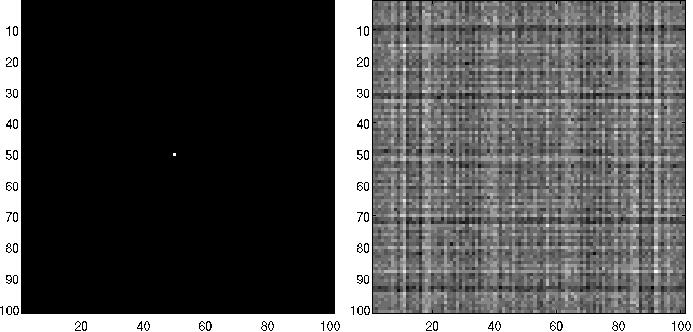
\includegraphics[width=10cm]{Figuras/Fig2_3.png}
   
\caption{Ejemplo de transformada de Fourier: $f(m, n) = 0 \; \; \forall (m, n) \neq (51, 51) \; \;  m, \; n \in [1, 101]$
         obtenido con plataforma MatLab$^{\textregistered}$ official license MathWorks 3407-8985-4332-9223-7918.}
\label{Fig2_3}

\end{figure}
\end{center}

\vspace{1.0cm}

\begin{center}
\begin{figure} [!h]

\centering
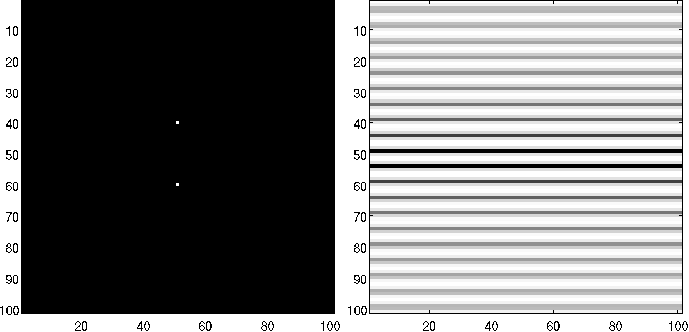
\includegraphics[width=10cm]{Figuras/Fig2_4.png}
   
\caption{Ejemplo de transformada de Fourier: $f(m, n) = 0 \; \; \forall (m, n) \neq (40, 51) \, \vee \neq (60, 51) \; \;  m, \; n \in [1, 101]$
         obtenido con plataforma MatLab$^{\textregistered}$ official license MathWorks 3407-8985-4332-9223-7918.}
\label{Fig2_4}

\end{figure}
\end{center}

\vspace{1.0cm}

\begin{center}
\begin{figure} [!h]

\centering
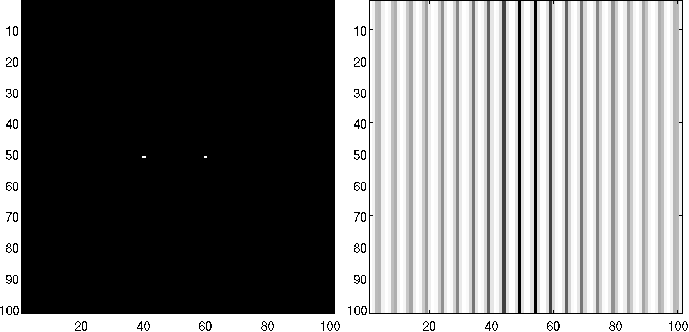
\includegraphics[width=10cm]{Figuras/Fig2_5.png}
   
\caption{Ejemplo de transformada de Fourier: $f(m, n) = 0 \; \; \forall (m, n) \neq (51, 40) \, \vee \neq (51, 60) \; \;  m, \; n \in [1, 101]$
         obtenido con plataforma MatLab$^{\textregistered}$ official license MathWorks 3407-8985-4332-9223-7918.}
\label{Fig2_5}

\end{figure}
\end{center}



\section{Filtros}
% \markboth{Intr. proc. im\'agenes radiol\'ogicas \'ambito m\'edico \ \textbf{M\'ODULO II}}{ESPECIALIDAD III \ \textbf{M\'ODULO II}}


A partir de las definiciones introducidas por las expresiones (\ref{EqL}) y (\ref{EqLI}) resulta posible realizar procesos de filtrado tanto en el dominio
especial de la imagen original $f(m, n)$ como en el dominio de las frecuencias de la transformada $F(m*, n*)$.
%

%
Una caracter\'istica significativa, que representa de hecho una de las principales ventajas de los espacios de transformadas, es que la operaci\'on de 
filtrado se realiza por medio de una multiplicaci\'on de transformadas; mientras que la operaci\'on en el espacio de coordenadas significa una convoluci\'on
denotada por el s\'imbolo $\otimes$. En virtud del teorema de convoluci\'on, se tiene:

\begin{eqnarray}
	f(m, n) \otimes g(m, n) = \int_{-\infty}^{\infty} \int_{-\infty}^{\infty} f(m, n) \; g(m-k, n-l)\; dk \, dl
\label{EqLII}
\end{eqnarray}

Aplicando la definici\'on de transformada de Fourier, se obtiene:

\begin{eqnarray}
	F_{f, g}(m*, n*) \equiv \mathbf{TF} [ f(m, n) \otimes g(m, n) ] =  \nonumber \\
	\mathbf{TF} [ f(m, n)] \; \mathbf{TF} [ g(m, n)] = F(m*, n*) \; G(m*, n*)
\label{EqLIII}
\end{eqnarray}

Para una dada funci\'on original $f(m, n)$ y su correspondiente transformada de Fourier $F(m*, n*)$, en referencia a la expresi\'on (\ref{EqLIII}) 
el operador $G(m*, n*)$ se define como un \textit{filtro espacial lineal} o \textit{funci\'on de transferencia} de filtro.
%

%
Entonces, la imagen resultado del proceso de filtrado $h(m, n)$ se obtiene aplicando la transformada inversa:

\begin{eqnarray}
	h(m, n) = \mathbf{TF^{-1}} [F_{f, g}(m*, n*) ]
\label{EqLIV}
\end{eqnarray}

El filtro queda determinado por medio de la funci\'on de transferencia o bien por la \textit{respuesta de impulso} $j(m, n)$ definida a partir de:

\begin{eqnarray}
	j(m, n) = F_{f, g}(m, n) = \delta (m, n) \otimes j(m, n) =  \nonumber \\
	\int_{-\infty}^{\infty} \int_{-\infty}^{\infty} \delta(m, n) \, j(k-m, l-n) \; dk \, dl
\label{EqLV}
\end{eqnarray}

Resulta que $j(m, n)$ es un filtrado intenso en t\'erminos de la funci\'on $\delta$ de Dirac.
%

%
A fines de c\'omputo, la transformada discreta de Fourier puede obtenerse, en modo an\'alogo a la expresi\'on (\ref{EqXLVIII}) operando:

\begin{eqnarray}
	F(m^*, n^*) = \mathbf{TF}[f(m, n)] = \frac{1}{M \, N} \sum_{m=0}^{M-1} \sum_{n=0}^{N-1} f(m, n) \; \nonumber \\
	\left[ \cos \left( 2 \pi  (\frac{m^* \, m}{M} + \frac{n^* \, n}{N}) \right) + 
	i \, \sin \left( 2 \pi  (\frac{m^* \, m}{M} + \frac{n^* \, n}{N}) \right)\right] \nonumber \\
	f(m, n) = \mathbf{TF^{-1}} [F(m^*, n^*)] = \sum_{m=0}^{M-1} \sum_{n=0}^{N-1} F(m^*, n^*) \; \nonumber \\
	\left[ \cos \left( -2 \pi  (\frac{m^* \, m}{M} + \frac{n^* \, n}{N}) \right) - 
	i \, \sin \left( 2 \pi  (\frac{m^* \, m}{M} + \frac{n^* \, n}{N}) \right)\right] \nonumber \\
\label{EqLVI}
\end{eqnarray}

Debido a la naturaleza discreta del espacio de muestreo intr\'inseco al procesamiento digital de im\'agenes, se determina la relaci\'on entre dominios 
espaciales y de frecuencias por medio de:

\begin{eqnarray}
	\Delta m^* = \frac{1}{M\; \Delta m}  \\
	\Delta n^* = \frac{1}{N\; \Delta n}
\label{EqLVII}
\end{eqnarray}

Cabe destacar que, por conveniencia de procesamiento, para el caso de im\'agenes ``cuadradas'' para las que $N = M$, se redefine la expresi\'on para la 
transformada de Fourier, multuplicando la expresi\'on (\ref{EqLVI}) por $N$, es decir:

\begin{eqnarray}
	F(m^*, n^*) = \mathbf{TF}[f(m, n)] = \frac{1}{N} \sum_{m=0}^{N-1} \sum_{n=0}^{N-1} f(m, n) \; 
	e^{-2 \pi \, i \, \left( \frac{m^* \, m + n^* \, n}{N} \right)} \nonumber \\
	f(m, n) = \mathbf{TF^{-1}} [F(m^*, n^*)] = \frac{1}{N} \sum_{m=0}^{N-1} \sum_{n=0}^{N-1} F(m^*, n^*) \; 
	e^{2 \pi \, i \, \left( \frac{m^* \, m + n^* \, n}{N} \right)} \nonumber \\
\label{EqLVIII}
\end{eqnarray}

La componente espectral compleja de $F(m^*, n^*)$ determina m\'odulo y fase, respectivamente, dados por:

\begin{eqnarray}
	\lvert F(m^*, n^*) \rvert = \sqrt{\left[ \Re{ \left( F(m^*, n^*) \right) }\right]^{2} + 
	\left[ \Im{\left( F(m^*, n^*) \right) } \right]^{2}} \nonumber \\ 
	\phi(m^*, n^*) = \arctan \left[ \frac{\Im{\left( F(m^*, n^*) \right) }}{\Re{\left( F(m^*, n^*) \right) }}\right]
\label{EqLIX}
\end{eqnarray}

donde $\Im$ y $\Re$ representan las componentes imaginaria y real, respectivamente.
%
Al filtrar una imagen original cuadrada $f(m, n)$ de dimensiones $N \times N$ mediante un filtro $j(m, n)$ de dimensiones $L \times L$ se obtendr\'a una 
imagen resultado $g(m, n)$ de dimensiones $N + L -1 \; \; \times \; \; N + L -1$.
%

%
Las propiedades de la transformada de Fourier permiten identificar de modo sencillo los operadores m\'as relevantes del procesamiento digital, como:
%

\vspace{1.0cm}

\underline{Operador de Traslaci\'on}

\vspace{0.5cm}

\begin{eqnarray}
	f(m, n)e^{2 \pi \, i (\frac{m^* _{0} \, m + n^* _{0} \, n}{N})} \leftrightarrow F(m^* - m^* _{0}, n^* - n^* _{0}) \\
	f(m - m_{0}, n - n_{0}) \leftrightarrow F(m^*, n^*) \, e^{-2 \pi \, i (\frac{m^* \, m_{0} + n^* \, n_{0}}{N})} \nonumber
\label{EqLX}
\end{eqnarray}

Es decir, una traslaci\'on al punto $(m_{0}, n_{0})$ se identifica con con el corrimiento del origen del plano del dominio de frecuencias al punto 
$(m^*_{0}, n^*_{0})$.
%
\vspace{1.0cm}

\underline{Operador de Rotaci\'on}

\vspace{0.5cm}

En coordenadas polares $m = \rho \, \cos{\theta} \; \; n = \rho \, \sin{\theta} \; \; m^* = \omega \, \cos{\phi} \; \; n^* = \omega \, \sin{\phi}$, las im\'agenes 
original $f(m, n)$ y transformada $F(m^*, n^*)$ son expresadas como $f(\rho, \theta)$ y $F(\omega, \phi)$.
%

%
Aplicando la definici\'on de transformada de Fourier, resulta:

\begin{eqnarray}
	f(\rho, \theta + \theta_{0}) \leftrightarrow F(\omega, \phi + \theta_{0}) 
\label{EqLXI}
\end{eqnarray}

Es decir, la rotaci\'on de la imagen original $f(\rho, \theta)$ (o $f(m, n)$) por un \'angulo $\theta_{0}$ se vincula con una rotaci\'on del mismo \'angulo en 
la imagen resultante $F(\omega, \phi)$ (o $F(m^*, n^*)$).
%

%
Las figuras \ref{Fig2_6} y \ref{Fig2_7} muestran ejemplos de aplicaci\'on de operadores de rotaci\'on, en dominio de coordenadas y de frecuencias, 
respectivamente.

\vspace{1.0cm}

\begin{center}
\begin{figure} [h!]

\centering
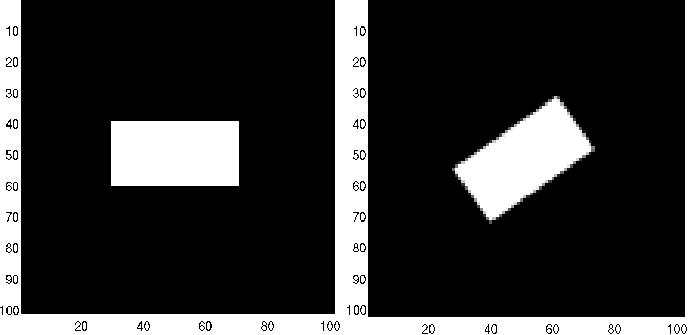
\includegraphics[width=8cm]{Figuras/Fig2_6.png}
   
\caption{Rotaci\'on de 35$^{o}$ de una imagen original $f(m, n)$ (o $f(\rho, \theta)$) obtenido con plataforma MatLab$^{\textregistered}$ official license MathWorks 3407-8985-4332-9223-7918.}
\label{Fig2_6}

\end{figure}
\end{center}

%\vspace{1.0cm}

\begin{center}
\begin{figure} [h!]

\centering
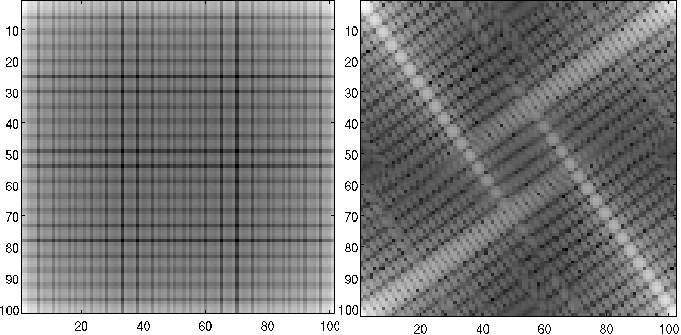
\includegraphics[width=8cm]{Figuras/Fig2_7.png}
   
\caption{Rotaci\'on de 35$^{o}$ de una imagen en dominio de transformada $F(m^*, n^*)$ (o $F(\omega, \phi)$)
         obtenido con plataforma MatLab$^{\textregistered}$ official license MathWorks 3407-8985-4332-9223-7918.}
\label{Fig2_7}

\end{figure}
\end{center}


%\vspace{1.0cm}

\underline{Operador de Escaleo}

\vspace{0.5cm}

La definici\'on de transformada de Fourier implica que $\mathbf{TF} [f_{A}(m, n) + f_{B}(m, n)] = 
\mathbf{TF} [f_{A}(m, n)] + \mathbf{TF}[f_{B}(m, n)]$ pero $\mathbf{TF} [f_{A}(m, n) \cdot f_{B}(m, n)] \neq 
\mathbf{TF} [f_{A}(m, n)] \cdot \mathbf{TF}[f_{B}(m, n)]$.
%

%
Sin embargo, para escalares $\alpha$ y $\beta$ se tiene:

\begin{eqnarray}
	\alpha \, f(m, n) \leftrightarrow \alpha \, F(m^*, n^*) \\
	f(\alpha m, \beta n) = \frac{1}{\lvert \alpha \beta \rvert} 
	F(\alpha \, m^*, \beta \, n^*)
\label{EqLXII}
\end{eqnarray}


\vspace{1.0cm}

\underline{C\'alculo de promedios}

\vspace{0.5cm}

El valor medio $\langle f \rangle$ se obtiene a partir de:

\begin{eqnarray}
	\langle f \rangle = \frac{1}{N^2} \sum _{m=0}^{N-1} \sum _{n=0}^{N-1} f(m, n)
\label{EqLXIII}
\end{eqnarray}

En particular, tomando $F(m^*=0, n^*=0)$ en la expresi\'on (\ref{EqLIX} (59)) se obtiene $ F(0, 0)= \frac{1}{N} \sum _{m=0}^{N-1} \sum _{n=0}^{N-1} f(m, n)$.
%
Por lo tanto, el valor promedio puede calcularse directamente a partir de:

\begin{eqnarray}
	\langle f \rangle = \frac{1}{N} F(m^* = 0, n^* = 0)
\label{EqLXIV}
\end{eqnarray}

\vspace{1.0cm}

\underline{C\'alculo de operadores de derivadas: OPerador de Laplace}

\vspace{0.5cm}

La laplaciana $\nabla^2$ de una imagen original $f(m, n)$ est\'a dada por:

\begin{eqnarray}
	\nabla^2 f(m, n) \equiv \frac{\partial^2}{\partial m^2} + \frac{\partial^2}{\partial n^2}
\label{EqLXV}
\end{eqnarray}

Aplicando la definici\'on de transformada de Fourier, se obtiene una expresi\'on \'util para el c\'alculo de la Laplaciana:

\begin{eqnarray}
	\mathbf{TF}[ \nabla^2 f(m, n) ] = -(2 \pi)^2 \left[ (m^*) ^2 + (n^*) ^2 \right] \; F(m^*, n^*)
\label{EqLXVI}
\end{eqnarray}









\subsection{Filtros de paso de banda}
% \markboth{Intr. proc. im\'agenes radiol\'ogicas \'ambito m\'edico \ \textbf{M\'ODULO II}}{ESPECIALIDAD III \ \textbf{M\'ODULO II}}

Las transiciones abruptas, como bordes y contornos, en una imagen original $f(m, n)$ se corresponden con altas frecuencias en el dominio de la
transformada.
%

\subsection{Filtros de suavizado}
% \markboth{Intr. proc. im\'agenes radiol\'ogicas \'ambito m\'edico \ \textbf{M\'ODULO II}}{ESPECIALIDAD III \ \textbf{M\'ODULO II}}

Puede aprovecharse esta caracter\'istica para implementar m\'etodos de filtrado para suavizar operando en el dominio de frecuencias.
%

%
Es posible suprimir frecuencias por debajo o por encima de valores pre determinados de manera que se produzcan efectos de suavizado seg\'un requerimientos.
%

\begin{center}
\underline{Filtros ideal de paso alto}
\end{center}

Consiste en la utilizaci\'on de la expresi\'on (\ref{EqLIII}) con la funci\'on de transferencia $G_{P\,A}(m^*, n^*)$ definida por:

\begin{eqnarray}
	G_{P\,A}(m^*, n^*) = \left\{ \begin{array}{ll} 
	0 & \mbox{$D(m^*, n^*) \leq D_{max}$}\\
	1 & \mbox{$D(m^*, n^*) > D_{max}$}.\end{array} \right.
\label{EqLXVII}
\end{eqnarray}

Para un valor m\'aximo de distancia $D_{max}$ como umbral para la distancia (independientemente de la m\'etrica), $D(m^*, n^*)$ es la distancia al 
origen de frecuencias $(m^* = 0, n^* = 0)$.
%

%
En el caso de la m\'etrica Euclidea $D(m^*, n^*) = \sqrt{ (m^*)^2 + (n^*)^2}$, el filtro se representa por un c\'irculo de radio $D_{max}$ como
muestra la figura \ref{Fig2_8}.

\vspace{1.0cm}

\begin{center}
\begin{figure} [!h]

\centering
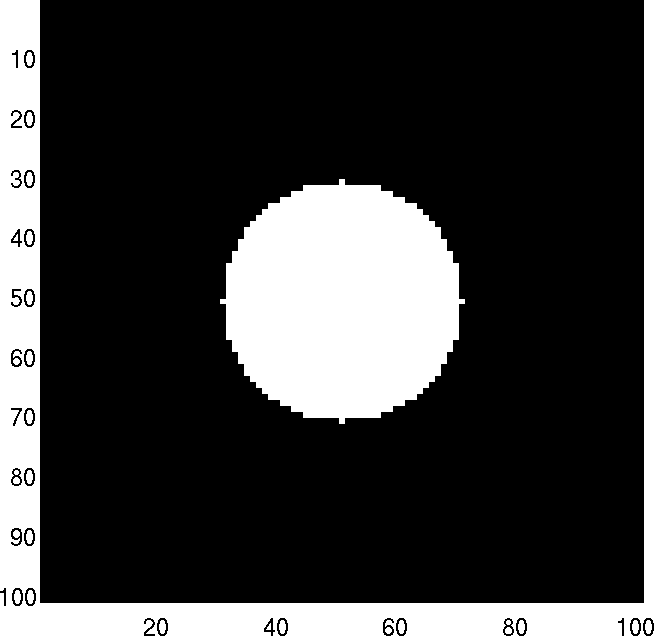
\includegraphics[width=8cm]{Figuras/Fig2_8.png}
   
\caption{Matriz de transferencia $G_{P\,A}$ para un filtro ideal de paso alto 
         obtenida con plataforma MatLab$^{\textregistered}$ official license MathWorks 3407-8985-4332-9223-7918.}
\label{Fig2_8}

\end{figure}
\end{center}

\begin{center}
\underline{Filtros ideal de paso bajo}
\end{center}

De modo an\'alogo, para el caso del filtro de paso bajo se define a partir de la matriz de transferencia $G_{P\,B}$ dada por:

\begin{eqnarray}
	G_{P\,B}(m^*, n^*) = \left\{ \begin{array}{ll} 
	1 & \mbox{$D(m^*, n^*) \leq D_{max}$}\\
	0 & \mbox{$D(m^*, n^*) > D_{max}$}.\end{array} \right.
\label{EqLXVIII}
\end{eqnarray}

La figura \ref{Fig2_9} muestra la matriz de transferencia de paso bajo $G_{P\,B}$.

\begin{center}
\begin{figure} [!h]

\centering
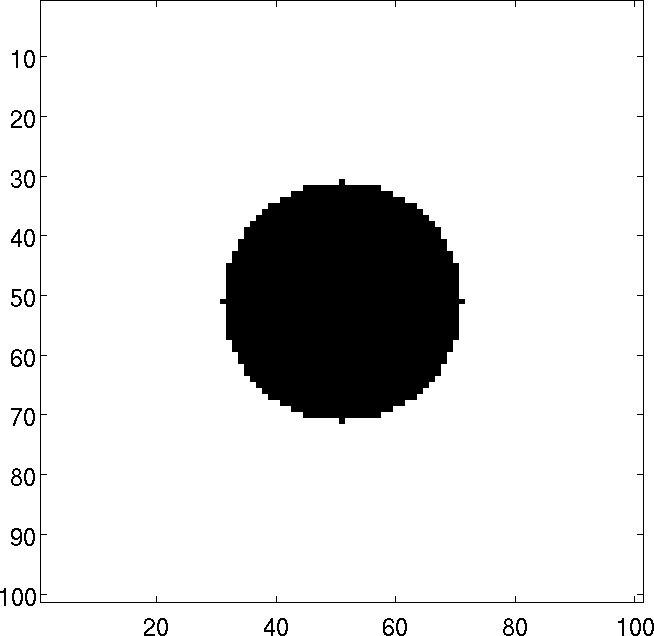
\includegraphics[width=8cm]{Figuras/Fig2_9.png}
   
\caption{Matriz de transferencia $G_{P\,B}$ para un filtro ideal de paso alto 
         obtenida con plataforma MatLab$^{\textregistered}$ official license MathWorks 3407-8985-4332-9223-7918.}
\label{Fig2_9}

\end{figure}
\end{center}

\subsection{M\'ascaras para filtrado}
% \markboth{Intr. proc. im\'agenes radiol\'ogicas \'ambito m\'edico \ \textbf{M\'ODULO II}}{ESPECIALIDAD III \ \textbf{M\'ODULO II}}

Una m\'ascara de filtrado $h(m, n)$ se denomina m\'ascara de convoluci\'on espacial si se define pormedio de:

\begin{eqnarray}
	F(m^*, n^*) = \frac{1}{N} \sum _{m=0}^{N-1} \sum _{m=0}^{N-1} h(m, n) \, e^{-2 \pi i \left( \frac{m^* \, m + n^* \, n}{N} \right)}
\label{EqLXIX}
\end{eqnarray}

Si la m\'ascara se restringue a una regi\'on espec\'ifica, tal que $h(m, n) = 0$ para $m \wedge n \ge N_{max} < N$ de modo que la m\'ascara restringida 
sea designada por $\hat{h}$, se obtiene:

\begin{eqnarray}
	\hat{H}(m^*, n^*) = \frac{1}{N} \sum _{n=0}^{N_{max}-1} \sum _{m=0}^{N_{max}-1} \hat{h}(m, n) \, 
	e^{-2 \pi i \left( \frac{m^* \, m + n^* \, n}{N} \right)}
\label{EqLXX}
\end{eqnarray}

De modo que puedan determinarse los coeficientes de la expansi\'on en (\ref{EqLXX}) que de minimizar la cantidad:

\begin{eqnarray}
	\chi^2 \equiv \sum _{m^*=0}^{N-1} \sum _{n^*=0}^{N-1} \lvert \hat{H}(m^*, n^*) - H(m^*, n^*) \rvert^2
\label{EqLXXI}
\end{eqnarray}

La expresi\'on anterior (\ref{EqLXXI}) puede resolverse por medio de una representaci\'on algebraica lineal $\mathbf{\hat{H}} = \mathbf{Q} \, \mathbf{\hat{h}}$ 
con $\mathbf{\hat{H}}$ representado por un vector de dimensi\'on $N^2$ cuyos elementos son los de $\hat{H}$ ordenados de alg\'un modo arbitrario, 
$\mathbf{\hat{h}}$ es un vector columna de dimensiones $N_{max}^2$ conteniendo los elementos de $\hat{h}$ y $\mathbf{Q}$ es una matriz de dimensiones
$N^2 \times N_{max}^2$ de t\'erminos exponenciales de acuerdo con la expresi\'on (\ref{EqLXIX}) dados por:

\begin{eqnarray}
	\mathbf{Q}(k, l) = q(k, l) = \frac{1}{N} e^{-2 \pi i \left( \frac{m^* \, m + n^* \, n}{N} \right)}
\label{EqLXXII}
\end{eqnarray}

para $k= m^* N + n^*$ con $m^* \wedge n^* \in [0, N-1]$ y $l= m N_{max} + n$ con $m \wedge n \in [0, N_{max}-1]$.

